% $Id: evaluation.tex 
% !TEX root = ../main.tex

\section{Empirical Study}
\label{sec:evaluation}

This section presents the empirical study for \flik. The purpose of the empirical study assessing the 
user experience and usefulness of \flik, when used to identify and locate bugs in  \ac{RL} programs. 
In particular, the participants were provided with three different \ac{RL} programs that implement three 
\ac{RL} problems. The problems were chosen according to their familiarity and an increasing 
environment complexity. 
\begin{enumerate*}[label=(\arabic*)]
\item GridWorld, is a standard benchmark for \ac{RL} based on episodic learning.
\item Rooms, is a common \ac{RL} problem with a similar structure to GridWorld, but with a higher 
complexity, used as an example of the possibility for agents to abstract their knowledge about the 
environment in hierarchical learning~\cite{pateria21} structures. 
\item Finally, Driving Assistant is a more recent \ac{RL} environment~\cite{cardozo18ml4pl,cardozo23}, 
uncommon to most developers, used to learn different tasks for autonomous driving in a continuous 
environment with more complex interaction between states, actions, and rewards. 
\end{enumerate*}

For the evaluation, a fault was manually injected in each program. The task assigned to the 
participants is to improve the functional quality of the three programs by removing the fault. Note that 
the injected bugs did not lead the program to exceptions or crashes, \ie each program run to 
completion, with no evident bug or strange behavior. The injected bugs caused the programs to 
produce outputs or agent behavior inconsistent with the expected outputs. 

For the empirical study the participants recruited are master and Ph.D. students that have taken the 
Reinforcement Learning course at Universidad de los Andes.  The participants are given a guide that 
describes the purpose of the tool, the task and steps, instructions on how to run and 
use \flik, documentation of the tool, and an small worked-out example. The problems implemented for 
the study are described in the following:\footnote{The evaluation guides and the information for the replication of the study are available at: \url{https://github.com/larodriguez22/Flik_Experiments}} 

%%%%
\paragraph{\textbf{GridWorld.}}
In its original presentation, the GridWorld environment is a standard benchmark for Q-learning, 
familiar to most \ac{RL} developers. For the study we use a larger GridWorld environment consisting 
of a $n \times m$ rectangular  board/grid ($10\times 10$ in our implementation), in which each tile 
$(i,j)$ represents a specific state of the board. Tiles in the board may be  walls, which agents cannot 
cross, or have a special exit status for agents to exit the board and terminate the episode. Exit tiles 
give a reward (positive of $1$ or negative of $-1$) to agents, as shown in \fref{fig:gridworld}. All tile 
types are unknown to the agent. The agent moves from a fixed starting point in the board, the top left 
corner at position $(0,0)$, searching for the goal state (\ie exit states with positive reward of $1$). The 
agent moves from state to state, avoiding  obstacles and undesired exit states (with a reward of $-1$). 

\begin{figure}[hptb]
  \centering
  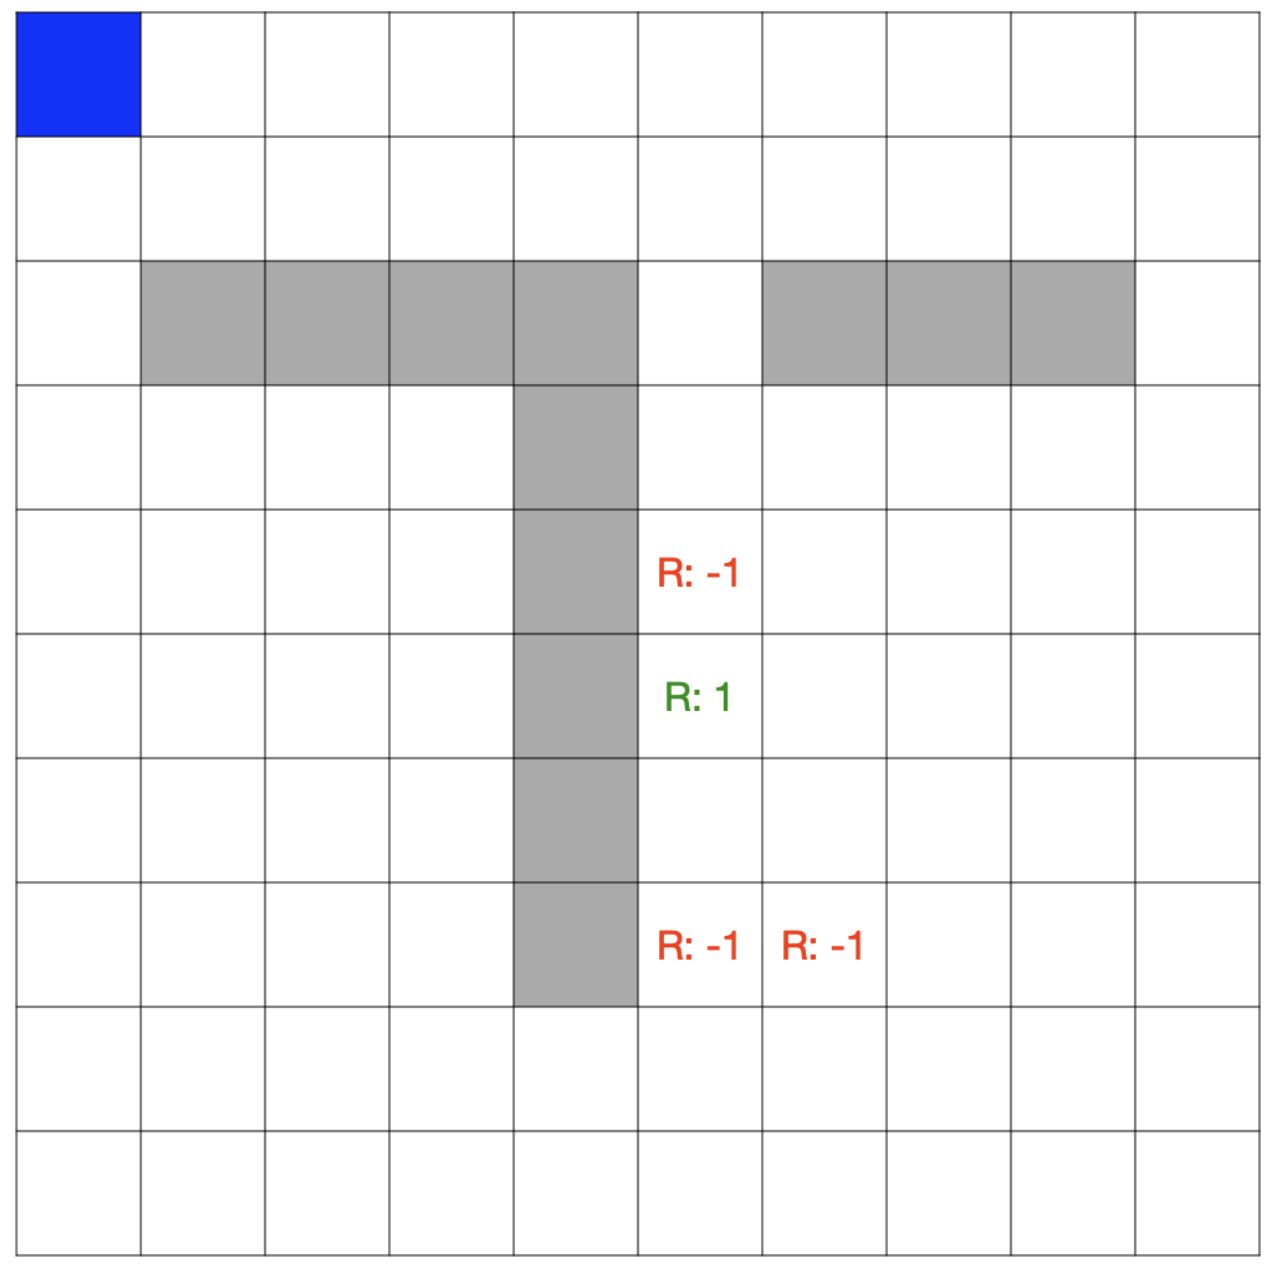
\includegraphics[width=0.5\columnwidth]{figures/gridworld.png}
  \caption{10x10 gridworld environment example}
  \label{fig:gridworld}
\end{figure}

The implementation of GridWorld introduces a bug in the definition of the $\epsilon$ hyperparameter, 
which leads to undesired behavior in the probability with which actions are taken by the agent, 
promoting exploitation without learning. The undesired behavior is given as the $\epsilon$ value is too 
small (\eg $0.1$) so that no or seldom exploration (taking a random action at each state) of the agent 
is allowed for the first couple of iterations. Afterwards, suing the epsilon decay strategy, the agent will 
consistently exploit the best action, which will be suboptimal if not wrong, to define its policy. This is 
an undesired behavior specially for training purposes as an agent should have a large probability to 
choose other actions and explore the grid. 

The objective of this task is that the study participants use \flik to navigate through the code and find 
out why the agent is not learning properly. Eventually, the participants should come out with the 
solution of increasing the value of $\epsilon$. 

%%%%
\paragraph{\textbf{Rooms.}} 
The four rooms maze environment has a similar composition to GridWorld, consisting of a 
$13\times 13$ board/grid divided in $4$ sections (\ie rooms), with walls between them, and a door 
opening to go from one room to another, as shown in \fref{fig:rooms}. The agent's objective in this 
environment is to exit through the upper-left room (the green square door in tile $(0,3)$) in the fewest 
possible number of steps. Reaching the exit state gives a reward of $1$ to the agent, and no 
other action gives a reward to the agent. In each episode the agent starts from any valid position in the 
grid, \eg the yellow square in the bottom-right room in the figure. 

\begin{figure}[hptb]
  \centering
  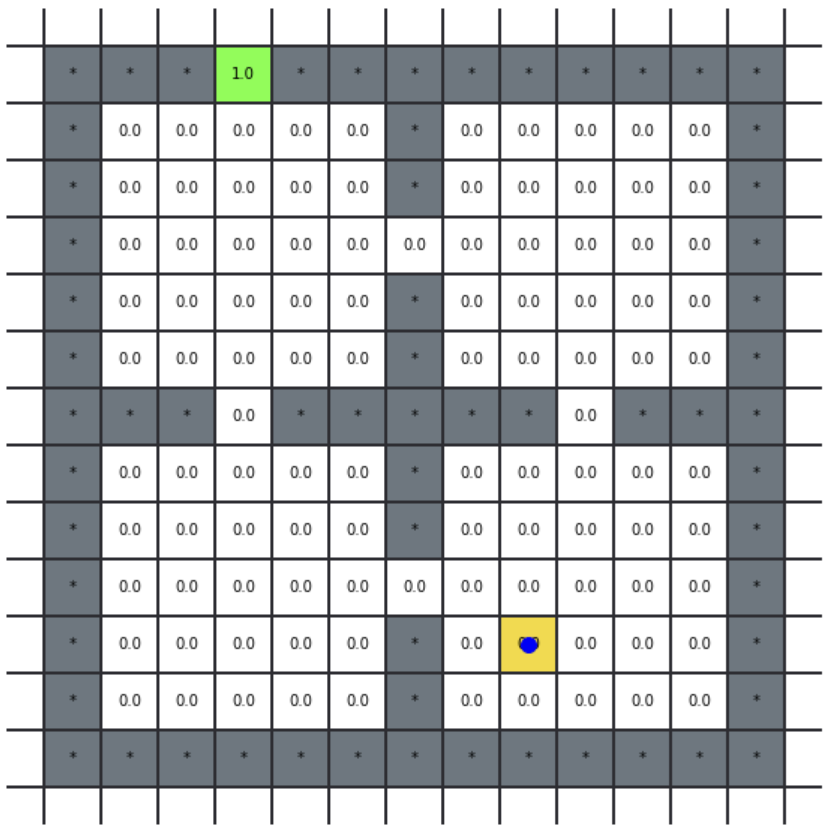
\includegraphics[width=0.5\columnwidth]{figures/rooms.png}
  \caption{Rooms environment example with associated rewards in each state}
  \label{fig:rooms}
\end{figure}

In this program, we introduced a bug in the implementation of the Bellman equation, exchanging the  
use of the the learning rate ($\alpha$) like:

\begin{itemize}
\item Original equation:
$
Q(s, a) \leftarrow (1-\alpha) Q(s, a) + \alpha \left( r + \gamma \max_{a'} Q(s', a') \right)
$

\item Erroneous equation implemented:
$
Q(s, a) \leftarrow  \alpha Q(s, a) + (1-\alpha) \left( r + \gamma \max_{a'} Q(s', a') \right)
$
\end{itemize}

In the original equation, $(1-\alpha) Q(s, a)$ is the current value and $\gamma \max_{a'} Q(s', a')$ 
is the maximum reward that can be obtained from state $s'$. This means that if the learning rate is 
very small the calculation of the current value will give a larger importance to the previously observed 
Q-values, leading to very little to no changes of the calculated Q-value. The effect of this behavior is 
that the agent learns short steps towards the optimal policy. In the Q-learning formula, the learning rate 
$\alpha$ defines how much old $Q(s,a)$ estimates are revised based on the new information. The 
learning rate ensures that, over time, the algorithm balances past knowledge with current learning, 
gradually incorporating new information while retaining important aspects of previous learning. 
Changing the equation in this way will disrupt the algorithm's balancing of previous and new 
knowledge. Specifically,$(1-\alpha)$ scales the difference between the new estimate and the old 
estimate. This makes the new information less influential as $\alpha$ gets larger, while the old value 
gets re-scaled by $\alpha$,  which does not align with the expected behavior of a Q-learning update. 

The objective of this task is that the participants use \flik to navigate through the code and find out 
the reason why the agent is not learning properly, afterwards we expected the participant to figure out
 a solution adjusting the proper value to update the Q-learning equation.

%%%%%%%
\paragraph{\textbf{Driving Assistant.}} 
The Driving Assistant environment focuses on an agent that must learn to drive, in a two lane road, by 
a given set of road rules. In this case, the agent is expected to learn to drive on the correct lane 
(determined by the reward), at the allowed speed, taking over slow traffic, and not crashing. 
The state of the environment is defines as a three tuple determined by the current speed of the vehicle, 
the current lane, and the proximity to the vehicle in front. To move in the environment, the agent has 
the following five possible actions to execute at every time-step: \spy{straight}, 
\spy{slow_down}, \spy{speed_up}, \spy{steer_left}, \spy{steer_right}. Finally, the agent receives  
negative rewards for the undesired behavior, $-800$ for crashing or coming to a full stop, $-600$ for 
driving too fast (over the $60Km/h$ speed limit), $-600$ for driving too slow (under $50Km/h$), 
$-500$ for driving on the wrong lane (the driving lane is the right lane of the road in our example). 
Additionally, the agent receives a reward of $50$ whenever there is no car in front.

Unlike the previous environment, study participants have not interacted with similar environments, 
not being a grid-based environment like GridWorld. Additionally, this environment is not episodic, as 
the vehicles can continuously drive. Nonetheless, the execution finishes and is immediately restarted 
upon a crash. \fref{fig:cars-code-example} shows the visual interface of this environment, where the 
agent's vehicle corresponds to the blue rectangle on top, and driving traffic is represented by red 
rectangles appearing either at the right lane (the driving lane at bottom of the interface), or the left lane 
(top of the interface).

\begin{figure}[hptb]
    \centering
    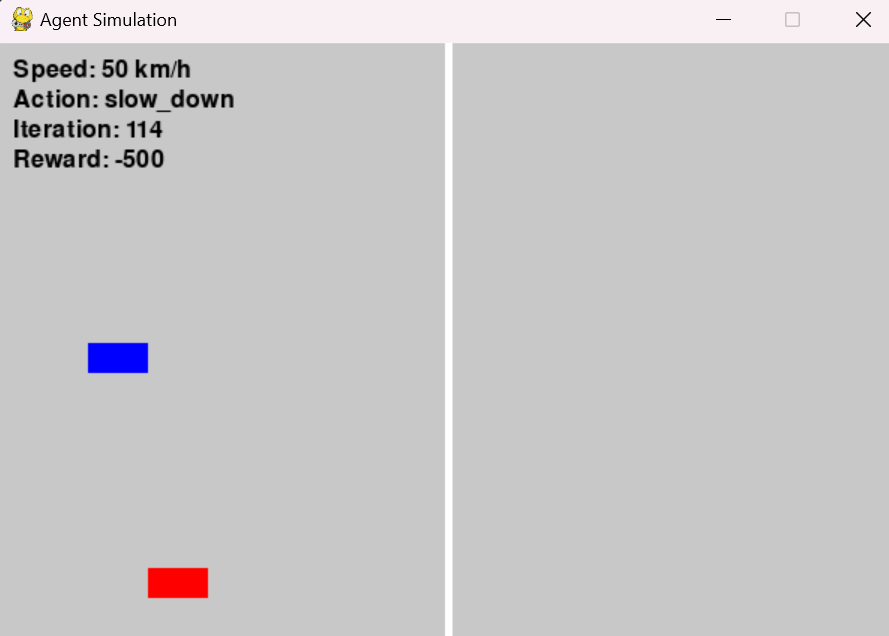
\includegraphics[width=0.5\textwidth]{figures/cars_example.png}
    \caption{Cars code example}
    \label{fig:cars-code-example}
\end{figure}

The bug introduced in this application is in the reward function, not motivating the agent to drive at 
the speed limit. The policy learned by the agent emerges as going very slowly or stopping altogether 
to avoid crashes, which is not the expected behavior. 

The objective of this task is that participants explore the program using \flik and observe the behavior 
of the reward and update it so that the agent can learn to drive appropriately as expected.
This is the largest task for the participants to analyze with \flik. 

%%%%%%
\paragraph{\textbf{Study conditions.}}
For the empirical study we had a session with 27 participants (\ie graduate students). 
The participants were asked to complete the three tasks (\ie GridWorld, Rooms, Driving Assistant)\footnote{The experiment environment, \flik, and the problems to solve are all available in a Docker distribution available through the Docker command \spy{docker pull lrodriguez22/py-flik-debugger:latest}} 
described previously. The full evaluation session used a time-slot of 1h30 split as follows: 
\begin{enumerate}[label=\textbf{\arabic*.}]
  \item During the first 20 minutes there the participants received a tutorial introduction to \flik and its 
  usage through a first example (long division) described in the evaluation guide.
  \item The following 50 minutes were used complete the three tasks, split into three blocks. 15 minutes 
  to finish the first task, 15 minutes to finish the second task, and  20 minutes to finish the third task. 
  \item At the end of the session, the participants were asked to fill an evaluation survey, for the 
  remaining 20 minutes. 
\end{enumerate}

The evaluation survey, defined as a google form, is divided in three sections: 
\begin{enumerate*}[label=(\arabic*)]
\item general knowledge questions, 
\item task questions, and 
\item usability of the tool questions.
\end{enumerate*}
The general knowledge questions are concerned with the participants' development experience 
(\ie using Python, debuggers and the terminal) to characterize participants. The task questions are 
concerned with the bug identified in each of the tasks, and the actions taken to fix it (if fixed). The 
usability questions are concerned with the participants' experience with the debugger, and additional 
feedback they could provide for improving \flik. The survey was anonymized. All the questions of the 
survey are inspired by similar empirical studies for debuggers, as for example the DeloreanJS 
back-in-time debugger for JavaScript~\cite{leger23}. All responses are available 
at \url{https://shorturl.at/DhN56}. 

The survey consisted of 23 multiple choice questions with a 5-points Likert scale, in which 5 means 
completely agree, and 1 means completely disagree. One of the questions was a yes or no question, 
to identify if the participants were willing to use the tool in the future. Finally, there were 10 open-answer 
questions, to dive deeper into feedback for the tool, and the tasks' complexity.


\endinput

